\documentclass[
    17pt,
    margin=1in,
    innermargin=-4.5in,
    blockverticalspace=-0.15in
]{tikzposter}
\geometry{paperwidth=42in,paperheight=30in}
\usepackage[utf8]{inputenc}
\usepackage{amsmath}
\usepackage{amsfonts}
\usepackage{amsthm}
\usepackage{amssymb}
\usepackage{mathrsfs}
\usepackage{graphicx}
\usepackage{subcaption}
\usepackage{adjustbox}
\usepackage{enumitem}
\usepackage{multirow}
\usepackage[american]{babel}
\usepackage{csquotes}
\usepackage[backend=biber,style=apa]{biblatex}
\DeclareLanguageMapping{american}{american-apa}
\usepackage{emory-theme}
\usepackage{inconsolata} % very nice fixed-width font included with texlive-full
\usepackage{color} % more flexible names for syntax highlighting colors
\usepackage{listings}
\lstdefinelanguage{julia}
{
  keywordsprefix=\@,
  morekeywords={
    exit,whos,edit,load,is,isa,isequal,typeof,tuple,ntuple,uid,hash,finalizer,convert,promote,
    subtype,typemin,typemax,realmin,realmax,sizeof,eps,promote_type,method_exists,applicable,
    invoke,dlopen,dlsym,system,error,throw,assert,new,Inf,Nan,pi,im,begin,while,for,in,return,
    break,continue,macro,quote,let,if,elseif,else,try,catch,end,bitstype,ccall,do,using,module,
    import,export,importall,baremodule,immutable,local,global,const,Bool,Int,Int8,Int16,Int32,
    Int64,Uint,Uint8,Uint16,Uint32,Uint64,Float32,Float64,Complex64,Complex128,Any,Nothing,None,
    function,type,typealias,abstract
  },
  sensitive=true,
  morecomment=[l]{\#},
  morestring=[b]',
  morestring=[b]" 
}

\definecolor{mygray}{RGB}{128,128,128}
\definecolor{myblue}{RGB}{0, 0, 255}
\definecolor{myolivegreen}{RGB}{186, 184, 108}
\definecolor{mymaroon}{RGB}{128, 0, 0}

\lstset{
    language=julia,
    basicstyle=\ttfamily, 
    columns=fullflexible, % make sure to use fixed-width font, CM typewriter is NOT fixed width
    numbers=left, 
    numberstyle=\small\ttfamily\color{mygray},
    stepnumber=1,              
    numbersep=10pt, 
    numberfirstline=true, 
    numberblanklines=true, 
    tabsize=4,
    lineskip=-1.5pt,
    extendedchars=true,
    breaklines=true,        
    keywordstyle=\color{myblue}\bfseries,
    identifierstyle=, % using emph or index keywords
    commentstyle=\sffamily\color{myolivegreen},
    stringstyle=\color{mymaroon},
    showstringspaces=false,
    showtabs=false,
    upquote=false
}

\makeatletter
\newcounter{tablecounter}
\newenvironment{tikztable}[1][]{
  \def \rememberparameter{#1}
  \vspace{10pt}
  \refstepcounter{tablecounter}
  \begin{center}
  }{
    \ifx\rememberparameter\@empty
    \else
    \\[10pt]
    {\small Table.~\thetablecounter: \rememberparameter}
    \fi
  \end{center}
}
\makeatother

\usepackage{mwe}    % for placeholder images

\addbibresource{refs.bib}

% Set theme parameters
\tikzposterlatexaffectionproofoff
\usetheme{EmoryTheme}
\usecolorstyle{EmoryStyle}

\title{AdvancedHMC.jl: a modular implementation of Stan’s no-U-turn sampler in Julia}
\author{Kai Xu\textsuperscript{1}, Hong Ge\textsuperscript{2}, Will Tebbutt\textsuperscript{2}, Mohamed Tarek\textsuperscript{3} and Martin Trapp\textsuperscript{4,5}}
\institute{
    \textsuperscript{1}University of Edinburgh \quad \textsuperscript{2}University of Cambridge \quad \textsuperscript{3}UNSW Canberra \quad \textsuperscript{4}Graz University of Technology \quad
    \textsuperscript{5}Austrian Research Institute for AI 
}
\titlegraphic{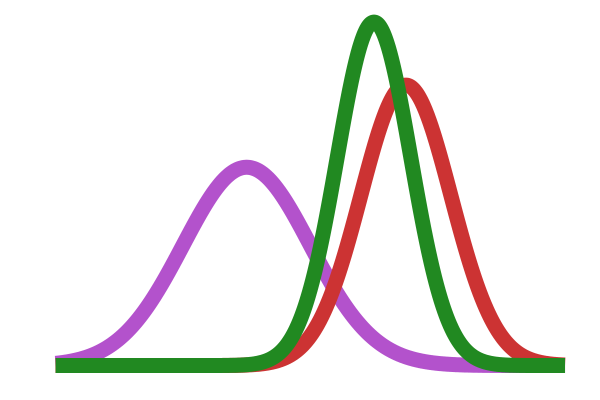
\includegraphics[width=0.075\textwidth]{turing-logo}}

% begin document
\begin{document}
\maketitle
\centering
\begin{columns}

\column{0.32}

\block{Abstract}{
    The No-U-Turn Sampler (NUTS) in Stan (\cite{hoffman2014no}) has demonstrated remarkable sampling robustness and 
    efficiency in a wide range of Bayesian inference problems, 
    due to the use of self-adaptive Hamiltonian dynamic trajectory simulation length, 
    together with a fine-tuned joint adaptation of step-size and mass matrix. 
    Motivated by these successes, we present 
    AdvancedHMC.jl (AHMC), a pure Julia implementation of Stan’s built-in NUTS and 
    related adaptation methods. 
    We hope AdvancedHMC.jl can expose Stan’s NUTS to a wider range of users, 
    e.g. those who want to write their models by hand, 
    or using a different probabilistic programming language (e.g. Turing, Soss). 
    In our package, NUTS is defined as a combination of individual components with 
    abstractions 
%  including the `Hamiltonian` dynamics, the `Metric` space, 
%  how the dynamics are numerically simulated by an Integrator to build up a `Trajectory`, 
%  and how a candidate point is sampled from it by a `TrajectorySampler`. 
%  This abstraction is partially 
    inspired by 
    (\cite{betancourt2017conceptual}).
    % A Conceptual Introduction to Hamiltonian Monte Carlo” by Michael Betancourt.
}

\block{Hamiltonian Monte Carlo Components}{
    Hamiltonian Monte Carlo (HMC) simulates Hamitonian dynamics to make proposals for a Markov chain (\cite{neal2011mcmc}).
    AdvancedHMC.jl supports the combination of various HMC samplers below.
    $$
    (StaticHMC \cup DynamicHMC) \times Adaptor.
    $$
    Here $StaticHMC$ are HMC with fixed-length trajectories and 
    $DynamicHMC$ are HMC with dynamic trajectories 
    which can be created by a combination of different NUTS components as follows
    $$
    Metric \times Integrator \times TrajectorySampler \times TerminationCriterion,
    $$
    where 
    \begin{equation*}
        \begin{aligned} 
            Metric &=  \{ UnitEuclidean, DiagEuclidean, DenseEuclidean \} \\ 
            Integrator &=  \{ Leapfrog \} \\
            TrajectorySampler &=  \{ Slice, Multinomial \} \\
            TerminationCriterion &= \{ ClassicNoUTurn, GeneralisedNoUTurn \}
        \end{aligned}.
    \end{equation*}
    $Adaptor$ contains any compositional adaptor composed from base adaptors
    $$
    BaseAdaptor \in \{Preconditioner, NesterovDualAveraging\}.
    $$

    \textbf{Note 1}: $Preconditioner$ behaves differently based on the choice of metric spaces.

    \textbf{Note 2}: a specific composition of base adaptors called $StanHMCAdaptor$ is provided to construct Stan's windowed adaptor, 
    which is proved to be robust in practice.
}

\block{Benchmark Models}{
    We use five models from MCMCBenchmarks.jl to compare 
    NUTS between AdvancedHMC.jl and Stan. \\

    \textbf{Gaussian Model (Gaussian)}
    is a simple two parameter Gaussian distribution.
    $$
    \mu \sim \mathcal{N}(0, 1), \quad 
    \sigma \sim \mathcal{T}runcated(\mathcal{C}auchy(0, 5), 0, \infty), \quad
    y_n \sim \mathcal{N}(\mu, \sigma) \; (n = 1, \dots, N)
    $$
    
    \textbf{Signal Detection Model (SDT)}
    is a model used in psychophysics and signal processing, 
    which decomposes performance in terms of discriminability and bias.
    $$
    d \sim \mathcal{N}(0, \frac{1}{\sqrt{2}}), \quad 
    c \sim \mathcal{N}(0, \frac{1}{\sqrt{2}}), \quad 
    x \sim \text{SDT}(d, c)
    $$
    
    \textbf{Linear Regression Model (LR)}
    is a linear regression with truncated Cauchy prior on the weights.
    $$
    B_d \sim \mathcal{N}(0, 10), \;
    \sigma \sim \mathcal{T}runcated(\mathcal{C}auchy(0, 5), 0, \infty), \;
    y_n \sim \mathcal{N}(\mu_n, \sigma),
    $$
    where $\mu = B_0 + B^T X, d = 1, \dots, D$ and $n = 1, \dots, N$. \\
    
    \textbf{Hierarchical Poisson Regression (HPR)}
    $$
    a_0 \sim \mathcal{N}(0, 10), \;
    a_1 \sim \mathcal{N}(0, 1), \;
    b_\sigma \sim \mathcal{T}runcated(\mathcal{C}auchy(0, 1), 0, \infty), \;
    b_d \sim \mathcal{N}(0, b_\sigma), \;
    y_n \sim \mathcal{P}oi(\log\lambda_n),
    $$
    where $\log\lambda_n = a_0 + b_{z_n} + a_1 x_n, d = 1, \dots, N_b$ and $n = 1, \dots, N$. \\
    
    \textbf{Linear Ballistic Accumulator (LBA)}
    is a cognitive model of perception and simple decision making.
    $$
    \tau \sim \mathcal{T}runcated(\mathcal{N}(0.4, 0.1), 0, mn), \quad
    A \sim \mathcal{T}runcated(\mathcal{N}(0.8, 0.4), 0, \infty),
    $$
    $$
    k \sim \mathcal{T}runcated(\mathcal{N}(0.2, 0.3), 0, \infty), \quad
    \nu_d \sim \mathcal{T}runcated(\mathcal{N}(0, 3), 0, \infty), \quad
    x_n \sim \text{LBA}(\nu, \tau, A, k)
    $$
    where $mn=\min_i x_{i,2}, d = 1, \dots, N_c$ and $n = 1, \dots, N$.
}

\column{0.36}

\block{Example Code of Building Stan's NUTS}{
    \lstinputlisting{example.jl}
}

\block{Sampling Efficiency: Stan v.s. AHMC}{
    To compare the sampling efficiency between Stan and AHMC,
    we run multiple runs of NUTS with target acceptance rate $0.8$ 
    for $2,000$ runs with $1,000$ adaptation steps,
    where the warm-up samples dropped off.
    Below are figures of distributions of step size and tree depth,
    and the mean effective sample size (ESS) for different variables.
    \begin{tikzfigure}[Gaussian (50 runs); left to right: step size, tree depth, ESS]
        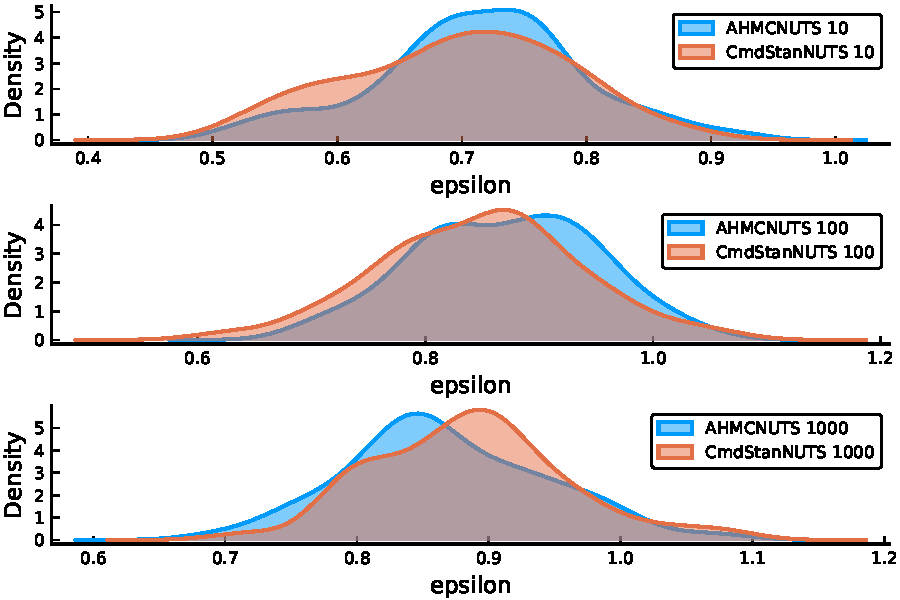
\includegraphics[width=0.08\textwidth]{./figs/Gaussian/density_epsilon.pdf}
        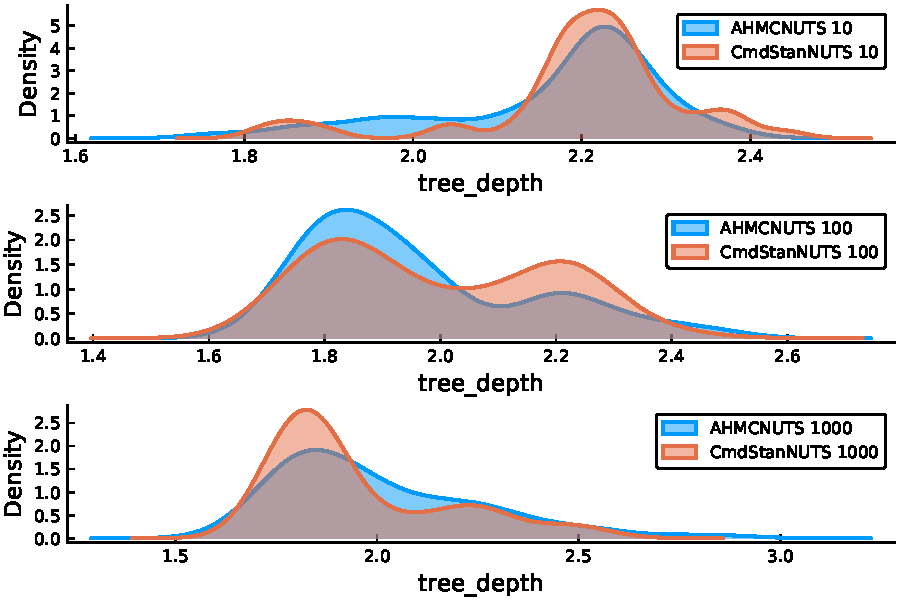
\includegraphics[width=0.08\textwidth]{./figs/Gaussian/density_tree_depth.pdf}
        \;
        \raisebox{\height}{\scalebox{0.75}{
            \begin{tabular}{llll}
                \multirow{2}{*}{Library} & \multirow{2}{*}{$N$} & \multicolumn{2}{c}{ESS} \\
                & & $\mu$ & $\sigma$ \\
                \hline \\
                Stan & 10 & 513.163 & 466.577 \\
                AHMC & 10 & 503.535 & 447.722 \\
                Stan & 100 & 786.531 & 782.231 \\
                AHMC & 100 & 786.531 & 796.628 \\
                Stan & 1000 & 864.01 & 876.66 \\
                AHMC & 1000 & 832.255 & 844.452 \\
            \end{tabular}
        }}
    \end{tikzfigure}
    \vspace{-2em}
    \begin{tikzfigure}[SDT (100 runs); left to right: step size, tree depth, ESS]
        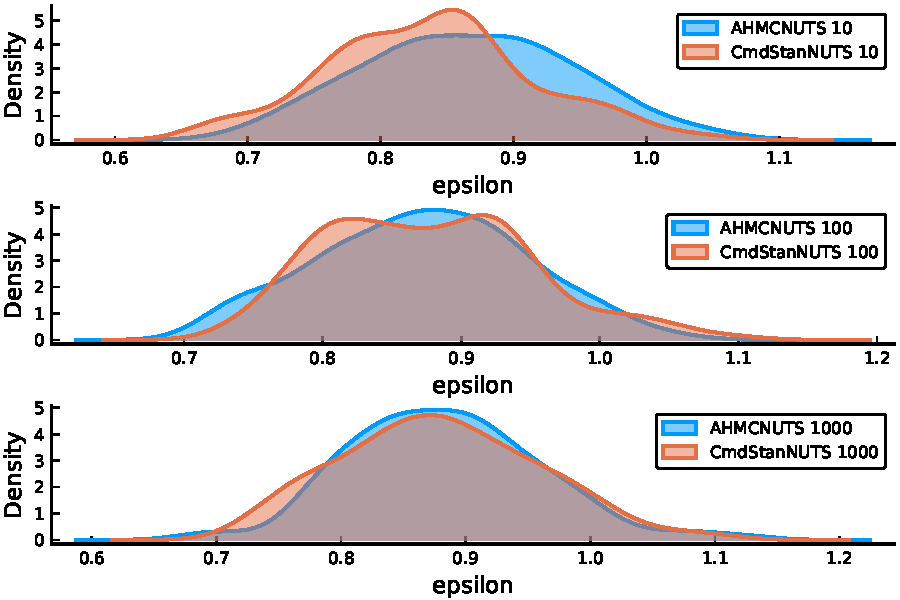
\includegraphics[width=0.08\textwidth]{./figs/SDT/density_epsilon.pdf}
        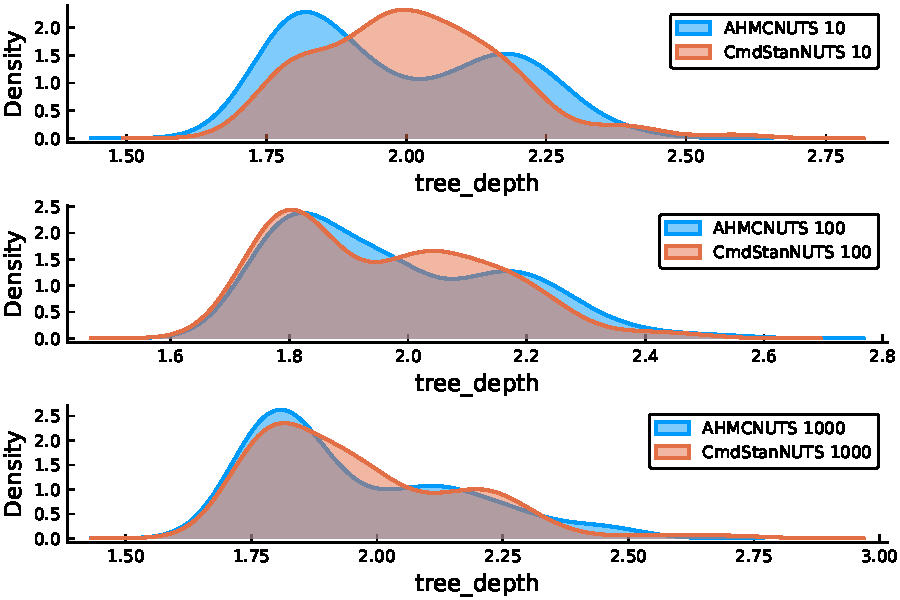
\includegraphics[width=0.08\textwidth]{./figs/SDT/density_tree_depth.pdf}
        \;
        \raisebox{\height}{\scalebox{0.75}{
            \begin{tabular}{llll}
                \multirow{2}{*}{Library} & \multirow{2}{*}{$N$} & \multicolumn{2}{c}{ESS} \\
                & & $d$ & $c$ \\
                \hline \\
                Stan & 10 & 710.762  & 703.327 \\
                AHMC & 10 & 802.236 & 815.929 \\
                Stan & 100 & 820.741 & 823.152 \\
                AHMC & 100 & 814.308 & 846.357 \\
                Stan & 1000 & 844.478 & 872.961 \\
                AHMC & 1000 & 829.792 & 859.018 \\
            \end{tabular}
        }}
    \end{tikzfigure}
    \vspace{-2em}
    \begin{tikzfigure}[LR (50 runs); left to right: step size, tree depth, ESS]
        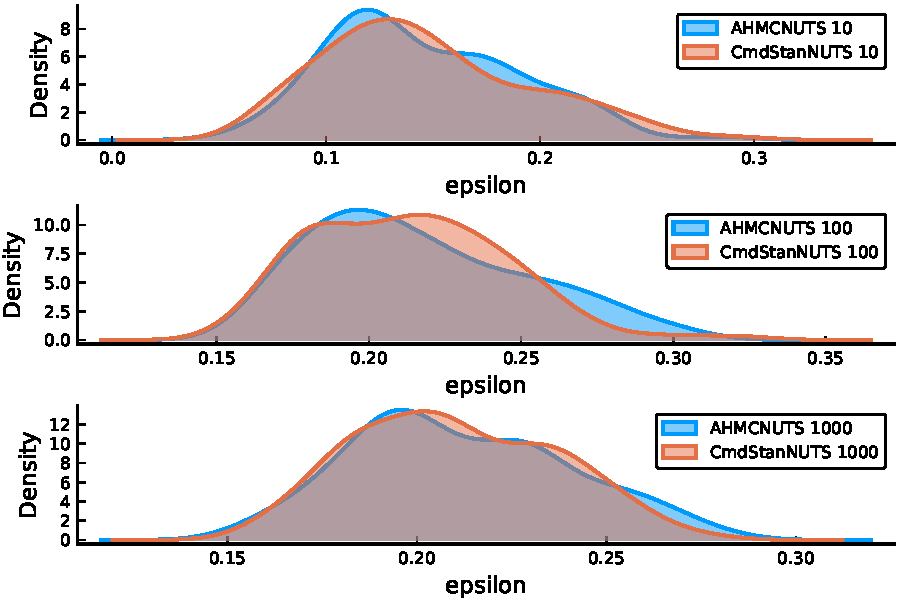
\includegraphics[width=0.08\textwidth]{./figs/Linear_Regression/density_epsilon.pdf}
        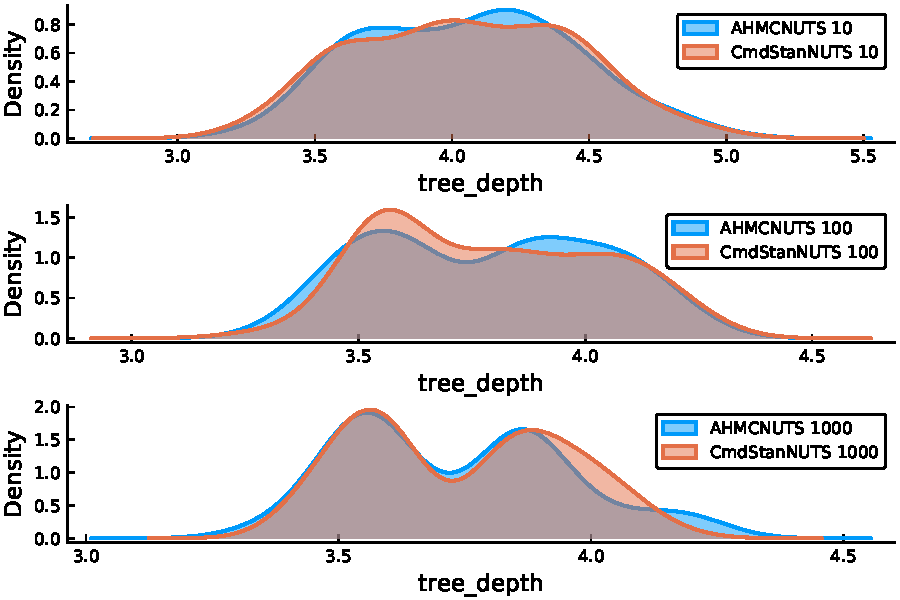
\includegraphics[width=0.08\textwidth]{./figs/Linear_Regression/density_tree_depth.pdf}
        \;
        \raisebox{\height}{\scalebox{0.75}{
            \begin{tabular}{llllll}
                \multirow{2}{*}{Library} & \multirow{2}{*}{$N$} & \multicolumn{4}{c}{ESS} \\
                & & $b_0$ & $\sigma$ & $b_1$ & $b_2$ \\
                \hline \\
                Stan & 10 & 413.939 & 266.476 & 381.219 & 423.441 \\
                AHMC & 10 & 354.946 & 263.894 & 411.769 & 399.42 \\
                Stan & 100 & 621.796 & 729.812 & 465.99 & 608.608 \\
                AHMC & 100 & 473.005 & 734.189 & 606.996 & 621.543 \\
                Stan & 1000 & 668.524 & 789.987 & 464.459 & 648.201 \\
                AHMC & 1000 & 485.988 & 786.577 & 676.097 & 689.344 \\
            \end{tabular}
        }}
    \end{tikzfigure}
    \vspace{-2em}
    \begin{tikzfigure}[HPR (25 runs); left to right: step size, tree depth, ESS (of some variables)]
        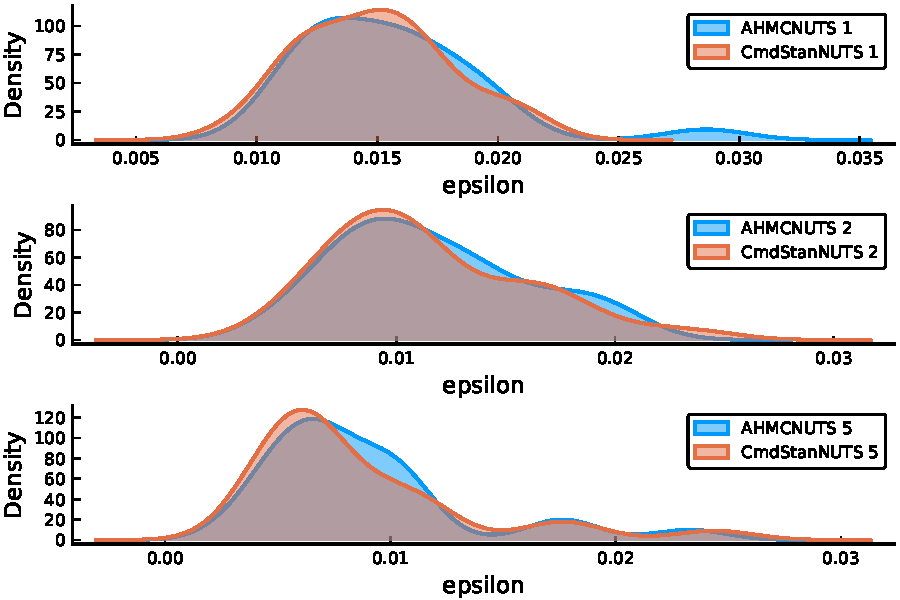
\includegraphics[width=0.08\textwidth]{./figs/Hierarchical_Poisson/density_epsilon.pdf}
        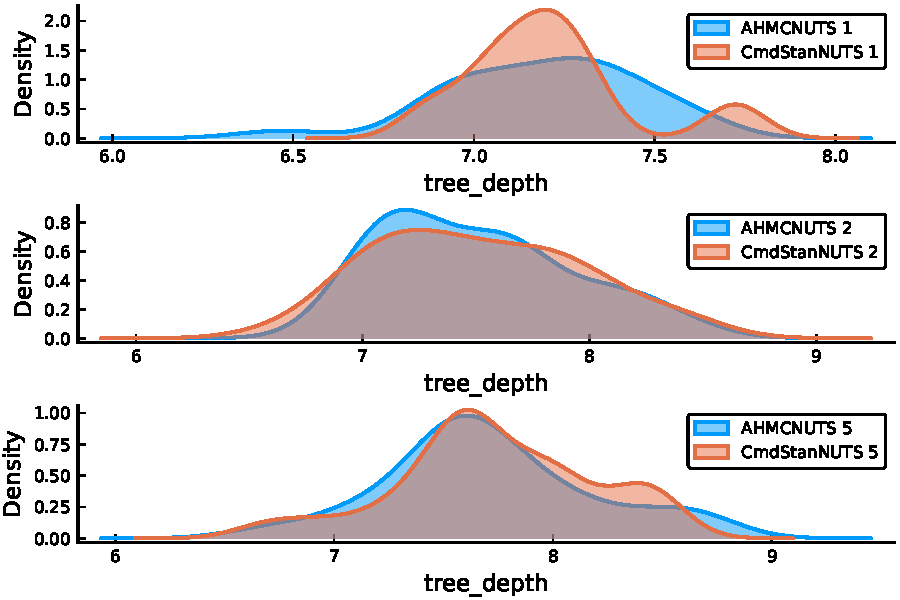
\includegraphics[width=0.08\textwidth]{./figs/Hierarchical_Poisson/density_tree_depth.pdf}
        \;
        \raisebox{\height}{\scalebox{0.75}{
            \begin{tabular}{lllll}
                \multirow{2}{*}{Library} & \multirow{2}{*}{$N$} & \multicolumn{3}{c}{ESS} \\
                & & $a_0$ & $a_1$ & $b_\sigma$ \\
                \hline \\
                Stan & 10 & 221.485 & 215.013 & 266.9 \\
                AHMC & 10 & 216.491 & 214.459 & 258.638 \\
                Stan & 20 & 208.286 & 207.041 & 241.08 \\
                AHMC & 20 & 206.458 & 200.469 & 236.546 \\
                Stan & 50 & 172.484 & 172.982 & 216.586 \\
                AHMC & 50 & 200.755 & 201.548 & 247.384 \\
            \end{tabular}
        }}
    \end{tikzfigure}
    \vspace{-2em}
    \begin{tikzfigure}[LBA (50 runs); left to right: step size, tree depth, ESS (of some variables)]
        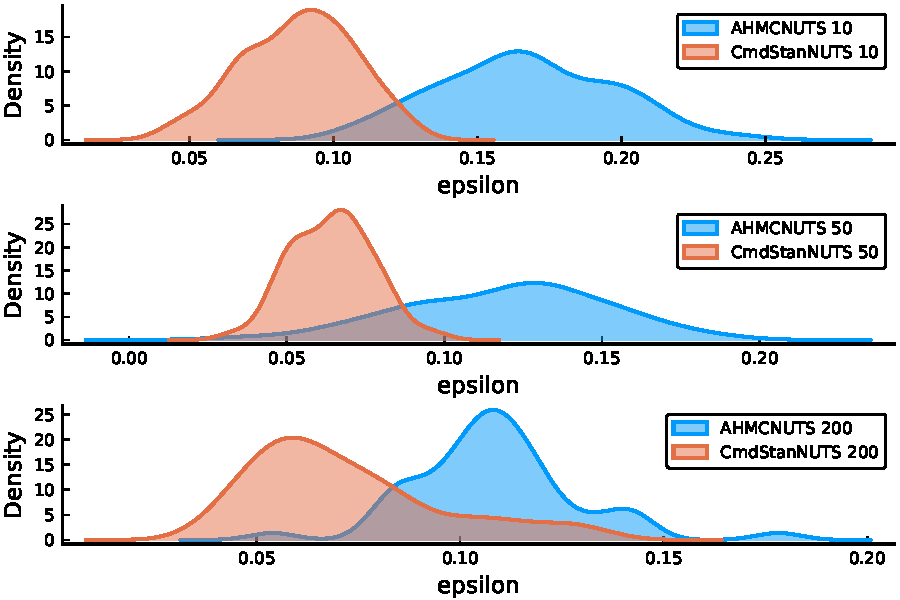
\includegraphics[width=0.08\textwidth]{./figs/LBA/density_epsilon.pdf}
        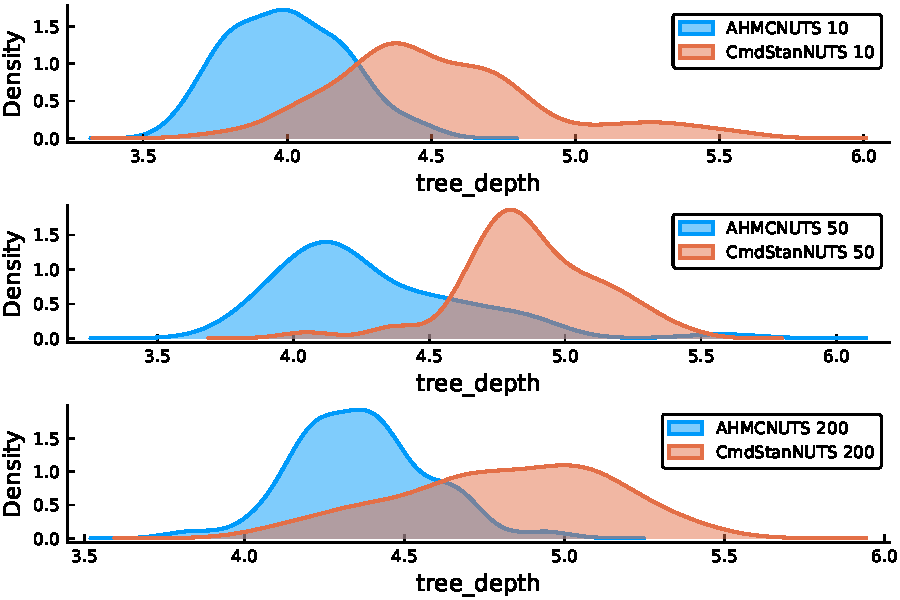
\includegraphics[width=0.08\textwidth]{./figs/LBA/density_tree_depth.pdf}
        \;
        \raisebox{\height}{\scalebox{0.75}{
            \begin{tabular}{llllll}
                \multirow{2}{*}{Library} & \multirow{2}{*}{$N$} & \multicolumn{4}{c}{ESS} \\
                & & $\tau$ & $A$ & $\nu_1$ & $\nu_2$ \\
                \hline \\
                Stan & 10 & 226.463 & 282.656 & 305.614 & 276.557 \\
                AHMC & 10 & 340.722 & 304.523 & 337.61 & 336.357 \\
                Stan & 50 & 212.838 & 238.003 & 235.009 & 232.667 \\
                AHMC & 50 & 248.249 & 238.979 & 248.331 & 255.421 \\
                Stan & 200 & 244.926 & 264.967 & 268.793 & 270.36 \\
                AHMC & 200 & 256.638 & 263.098 & 270.978 & 266.769 \\
            \end{tabular}
        }}
    \end{tikzfigure}
}

\column{0.32}
\block{Computational Efficiency: Stan v.s. Turing}{
    \textbf{Turing.jl} is a probabilistic programming language (PPL) in Julia that
    uses AdvancedHMC.jl as its HMC backend.
    All the benchmark models are written in Turing and AdvancedHMC.jl
    is called by Turing.jl to run the NUTS.
    Below is an example of running NUTS on the LR model using Turing.
    \lstinputlisting{lr.jl}    
    The time to run the five benchmark models in Stan and Turing
    are reported in the table below.
    \begin{tikztable}[Time comparisons between Stan and AdvancedHMC.jl for five models]
    \begin{tabular}{l|ll|ll|ll|ll|ll}
        \multirow{2}{*}{Library} & \multicolumn{10}{c}{Data Size \& Mean Time (s)} \\
        & \multicolumn{2}{c}{Gaussian (50 runs)} & \multicolumn{2}{c}{SDT (100 runs)} & \multicolumn{2}{c}{LR (50 runs)} & \multicolumn{2}{c}{HPR (25 runs)} & \multicolumn{2}{c}{LBA (50 runs)} \\
        % \hline \\
        Stan & 10 & 0.803881 & 10 & 0.775959 & 10 & 0.866924 & 10 & 2.487 & 10 & 1.91799 \\
        AHMC & 10 & 0.336073 & 10 & 0.328538 & 10 & 1.13563 & 10 & 19.4587 & 10 & 2.69062 \\
        Stan & 100 & 0.756092 & 100 & 0.726106 & 100 & 0.982419 & 20 & 3.50248 & 50 & 7.84705 \\
        AHMC & 100 & 0.33034 & 100 & 0.320111 & 100 & 1.32024 & 20 & 28.2982 & 50 & 11.027 \\
        Stan & 1000 & 0.761393 & 1000 & 0.708934 & 1000 & 2.26 & 50 & 5.89541 & 200 & 31.3762 \\
        AHMC & 1000 & 0.508123 & 1000 & 0.317854 & 1000 & 3.83261 & 50 & 40.0322 & 200 & 33.6125 \\
    \end{tabular}
    \end{tikztable}
}

\block{Easy Integration of Other Julia Packages}{
    \textbf{Bijectors.jl} is used inside Turing.jl to do automatic transformation of constrained variables in order to run HMC.
    E.g. a random variable from $\mathcal{T}runcated(\mathcal{C}auchy(0, 5), 0, \infty)$ is constrained to be positive and 
    will be transformed to the real space by the $\log$ function automatically. \\
    
    \textbf{CuArrays.jl} could be used with AdvancedHMC.jl to run NUTS on GPUs.
    In order to run NUTS using CUDA, 
    one only needs to change Line 3 of the demo code 
    from \texttt{q\_init = randn(D)} to \texttt{q\_init = CuArray(randn(D))}, 
    assuming \texttt{logdensity\_f} and \texttt{grad\_f} in Line 6 are GPU friendly;
    if they are written in pure Julia, they probably supports GPUs automatically. \\
    \textit{How does it work?}
    All arrays in AdvancedHMC.jl are typed as \texttt{AbstractArray} and
    the concrete type will be inferred from the initial parameter \texttt{q\_init}.
    That is to say, if the initial parameter is on GPU, i.e. a \texttt{CuArray},
    all the internal arrays in AdvancedHMC.jl will be on GPU, so does the NUTS. \\

    \textbf{SoSS.jl} is another probabilistic programming language in Julia that
    supports AdvancedHMC.jl as its backend.
    It is easy for PPLs in Julia with different domain specific languages (DSLs)
    to use the HMC implementation in AdvancedHMC.jl. \\

    \textbf{DifferentialEquations.jl} is a suite for numerically solving differential equations in Julia 
    with efficient implementations of solvers for various differential equations.
    The solvers can be directly used in the Turing model and 
    perform Bayesian inference on parameters of differential equations. \\

    \textbf{Flux.jl} is a deep learning packages in Julia.
    Neural models defined by Flux.jl can be directly used in Turing models.
    E.g. one can implement a Bayesian neural network in Turing by 
    defining priors on the weights of a Flux-based neural network, and 
    NUTS can be used to draw samples of the weights.
}

\block{Acknowledgements}{
    We would like to thank the developers of MCMCBenchmarks.jl, Rob Goedman and Christopher Fisher.
    With this package we run all the benchmarks and generate all the plots used in this poster.
    % We would also like to thank Martin Trapp for useful discussions on efficient implementations of the benchmark models in Turing.jl.
}

\block{References}{
    \vspace{-1em}
    \printbibliography[heading=none]
}
    
\end{columns}
\end{document}